\section{Ethics}
	\subsection{Grundbegriffe}
	
		\begin{longtable}{|>{\bfseries}p{0.2\textwidth}||p{0.75\textwidth}|}
			\hline
			Begriff
				& \textbf{Erklärung}\\
			\hhline{|=#=|}
			Sozialtheorie
				& Stellt sich die Frage "Wie sollen wir leben?".\\
			\hline
			Glückstheorie
				& Stellt sich die Frage "Was ist ein gutes, gelingendes, glückliches Leben?".\\
			\hline
			Handlungstheorie
				& Stellt sich die Frage "Was heisst verantwortungsvolles Handeln?".\\
			\hline
			Gerechtigkeitstheorie
				& Stellt sich die Frage "Was heisst Gerechtigkeit?".\\
			\hline
			Moral
				& Beschreibt das Normen- und Wertesystem, welches sich aus einer kulturellen Tradition entwickelt hat.\\
			\hline
			Ethik
				& Theorie, die sich mit der Moral beschäftigt. Sie fragt grundlegend nach einem gelingenden, glücklichen Leben.\\
			\hline
			Ethos
				& Gewohnheit, Sitte, Brauch bzw. Charakter, Seelenzustand\\
			\hline
			Deskriptive Methode
				& Hält die faktische Handlungs- und Verhaltensweise, die Wertvorstellungen und Geltungsansprüche einer Gesellschaft fest, ohne sie zu werten.\\
			\hline
			Normative Methode
				& Vorschreibendes Verfahren, welches universell gültige Regeln der Ethik sucht.\\
			\hline
			Relativismus
				& Bezieht seine Aussagen auf soziale, kulturelle, historische oder persönliche Gegebenheiten zurück.\\
			\hline
			Universalismus
				& Will universell gültige Aussagen machen, ohne dabei auf soziale, kulturelle, historische oder persönliche Unterschiede zu achten.\\
			\hline
			Metaphysik
				& Eine Grunddisziplin der Philosophie, welche die Fundamente, Voraussetzungen, Ursachen, Gesetzlichkeiten und Prinzipien, sowie Sinn und Zweck der gesamten Realität behandelt.\\
			\hline
			Kategorischer Imperativ
				& ''Handle nur nach derjenigen Maxime, durch die du zugleich wollen kannst, dass sie ein allgemeines Gesetz werde.'' - Immanuel Kant (Kant's grundlegendes Prinzip der Ethik)\\
			\hline
			Sophistik
				& Bewegung in der griechischen Antike, in welcher ihre Vertreter (die Sophisten) ihr Wissen an andere vermittelten. Meist gegen Bezahlung an Staatspersonen und Adelige.\\
			\hline
			Forderungen an die Philosophie
				& Suche nach guten, für andere Personen einsehbare Argumenten, die keine Widersprüche Enthalten und den Erfahrungen entsprechen.\newline
					Nicht akzeptiert sind Offenbarungen, Erleuchtungen und blosse Behauptungen.\\
			\hline
		\end{longtable}
		
	\subsection{Vergleich der behandelten Philosophen}
		
		\subsubsection{Platon}
			\begin{longtable}{>{\bfseries}p{0.25\textwidth}p{0.7\textwidth}}
				\hline
				Geboren
					& \\
				\hline
				Gestorben
					& \\
				\hline
				Fokus der Fragestellungen
					& Theoretische, defintorische Grundlegungen.\\
				\hline
				Fragetyp
					& ''Was ist X?'', e.g ''Was ist Tugend?''\newline
						\textrightarrow\ sehr schwierig zu beantworten, da man nicht weiss ob eine Beschreibung von X korrekt ist, wenn man nicht weiss was X genau ist.\\
				\hline
				Stand zu Sophisten
					& Kritisierte die Sophisten radikal.\newline
					  Gemäss den Sophisten ist ''Gut, was für mich gut ist''.\newline
					  Sokrates hingegen fand ''Gut, was für mich gut ist, und was für die anderen gut ist''.\newline
					  Appellierte an Wissensträger, ihr Wissen weiterzuleiten.\newline
					  Der aufgeklärte Zustand soll die ganze Stadt erreichen, durch ''Überredung und Zwang''.\\
				\hline
				Höhlengleichnis
					&	\vspace{0pt}
						
						\begin{minipage}{0.75\textwidth}
							\begin{figure}[H]\centering
								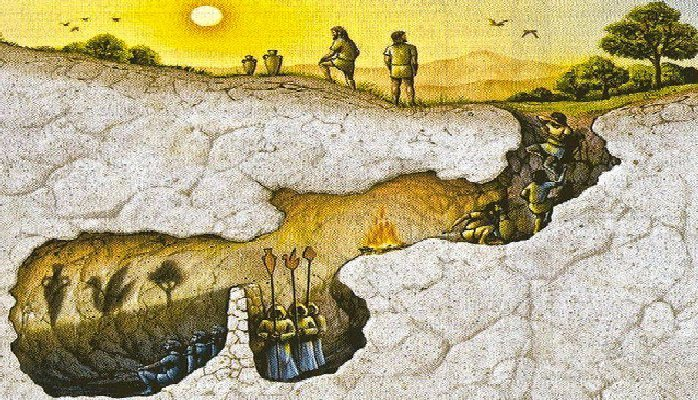
\includegraphics[scale=0.4]{./pictures/hoehlengleichnis.jpeg}
							\end{figure}
						\end{minipage}\\
					& Gespräch zwischen Sokrates (Gesprächsleiter) und Glaukon (Schüler von Sokrates), festgehalten von Platon.\\
					& \textbf{\underline{Erster Teil:}}\newline
						
						Ganzes Leben gefesselt in einer Höhle, so dass man nur n die Wand sehen kann.\newline
						Am Eingang der Höhle brennt ein Feuer.
						Zwischen dem Feuer und dem Gefangenen führt ein Weg, entlang welchem eine Mauer verläuft.\newline
						Gaukler tragen Gegenstände über die Mauer. (Falsche Realität vorgaukeln)\newline
						Man sieht nur deren Schatten, und hört Stimmen von einzelnen Gauklern.\newline
						Stimmen werden den Schatten zugesprochen.\newline
						Das einzige, was man für wahr empfindet, sind die Schatten, und die Stimmen welche von den Schatten stammen.\newline
						
						 \textbf{Hauptbotschaft:} Wir leben oft in einer falschen Vertrautheit, und in einer falschen Sicht auf uns selbst. Nur aussergewöhnliches wird hinterfragt.
						\\
					& \textbf{\underline{Zweiter Teil:}} \newline
						Könnte sich ein Gefangener befreien, würde er vom Feuer geblendet, er wäre verwirrt, und der Aufstieg aus der Höhle wäre anstrengend.\newline
						Ein Gefangener wird entfesselt und aus der Höhle gezerrt.\newline
						Gefangener ist am Höhlenausgang und erblickt zuerst das Feuer, und dann die Sonne selbst.\newline
						Gefangener erfährt zum ersten Mal neue Realität und muss seine Erfahrungen in Frage stellen.\newline 
						Gefangener begibt sich wieder in die Höhle zu den anderen Gefangenen.\newline
						Gefangener ist an das Sonnenlicht gewöhnt, und erkennt in der Höhle die Schatten kaum mehr.\newline
						Gefangener wirkt für andere Gefangene dumm.\newline
						Andere Gefangene denken,dass der Aufstieg aus der Höhle die Augen verderben\newline
						
						 \textbf{Hauptbotschaft:} Wenn man an Vorurteile und Täuschungen gewöhnt ist, ist ein ''Aufstieg aus dieser Gefangenschaft'' schwierig. Kritisches denken benötigt einen Trieb, und es herrscht oft ein Widerstand dagegen.
						\\
			\hline
			Ideenlehre
				& Auch ''Zwei-Welten-Lehre''\newline
					Heftig umstritten.\newline
					Welt ist klar unterteilt in:
					\begin{itemize}
					  \item Erfahrungswelt (\textbf{''Welt des Werdens''}): vergänglich \& ambivalent, mit Sinnen wahrgenommen.
					  \item Ideenwelt (auch \textbf{''Welt des Seins''}):	enthält das Wahre, Gute, Schöne und Ewige. Ideen sind unveränderlich.
					\end{itemize}
					
					Die Ideenwelt nimmt Göttliche und vollkommene Züge an. Vor dem Leben in der Erfahrungswelt lernt der Geist die Ideen schon kennen, und kann sich in der Erfahrungswelt an sie erinnern. Er darf sich nur nie aufhören, daran zu erinnern. Der Schritt von der Erfahrungswelt in die Ideenwelt wird gewährt, wenn man ein ethisches Leben führt.\\
				& \underline{Beispiel des Schreiners:}\newline
					Schreiner findet in seinem Geiste Form und Gestalt eines vollkommenen Tisches vor.\newline
					Er hat die Form nicht geschaffen, nur gefunden.\newline
					Hinblickend auf diesen Tisch fertigt er beliebig viele Tische (Material auch gegeben).\newline
					Diese Tische sind Abbilder des einen urbildlichen Tisches.\\
				& Weiterentwicklung zweier vorsokratischer Denkansätze:
					\begin{itemize}
					  \item Heraklit: Welt eines permanenten Wandels (''Alles Fliesst'', ''Du steigst niemals zweimal in den gleichen Fluss'').
					  \item Parmenides: Welt des starren Seins.
					\end{itemize}\\
				\hline														 
			\end{longtable}
			
			
		\subsubsection{Sokrates}
			\begin{longtable}{>{\bfseries}p{0.25\textwidth}p{0.7\textwidth}}
				\hline
				Geboren
					& \\
				\hline
				Gestorben
					& \\
				\hline
				Literatur
					& Hat keine Texte selbst verfasst.\newline
						Nur seine Schüler, insbesondere Platon, haben sein Gedankengut festgehalten.\\
				\hline
				Methode
					& Hat sich Gesprächspartner auf den Strassen und Plätzen von Athen gesucht, und zwang sie durch hartnäckige Fragen, über Dinge nachzudenken, die ihnen bis anhin selbstverständlich erschienen.\newline
						Er dachte, dass er so das Wissen ans Licht brachte, dass im Partner schon verborgen vorhanden gewesen ist.\\
				\hline
				Platon's Höhlengleichnis
					& Sokrates stellt höchste Ansprüche an die Philosophie, damit eine gerechte Gesellschaft heranwachsen kann. Die Aufklärung der anderen ist wichtig, und wenn man Gelehrte dazu nötigt, ist dies kein Unrecht, sondern eine gerechte Zumutung.\\
				\hline
			\end{longtable}	
			
			
		\subsubsection{Aristoteles}
			\begin{longtable}{>{\bfseries}p{0.25\textwidth}p{0.7\textwidth}}
				\hline
				Geboren
					& \\
				\hline
				Gestorben
					& \\
				\hline
				Ethik-Typ
					& Tugendethik\\
				\hline
				Fokus der Fragestellungen
					& Praktische Folgen einer Handlung.\\
				\hline
				Höchste Tugend
					& Weisheit\\
				\hline
				Weitere wichtige Tugenden
					&	
					\begin{itemize}
						\item Gerechtigkeit
						\item Tapferkeit
						\item Mässigung
						\item Freigebigkeit
						\item Hilfsbereitschaft
						\item Sanftmut
						\item Wahrhaftigkeit
						\item Höflichkeit
						\item Einfühlsamkeit
					\end{itemize}\\
				\hline
				Höchstes Gut/Ziel
					& Glücklichsein. Er behauptet, dass dies erarbeitet werden kann.\\
				\hline
			\end{longtable}	
		
		\subsubsection{Immanuel Kant}
			\begin{longtable}{>{\bfseries}p{0.25\textwidth}p{0.7\textwidth}}
				\hline
				Geboren
					& \\
				\hline
				Gestorben
					& \\
				\hline
			\end{longtable}	

% 		\begin{longtable}{|p{0.1\textwidth}||p{0.2\textwidth}|p{0.2\textwidth}|p{0.2\textwidth}|p{0.2\textwidth}|}
% 			\hline
% 				& Aristoteles
% 				& Sokrates
% 				& Platon
% 				& Immanuel Kant \\
% 			\hhline{|=#=|=|=|=|}
% 			Grundidee
% 				&
% 				&
% 				&
% 				& \\
% 			\hline
% 			Ethik-Typ
% 				& Tugendethik
% 				& Deontologische Ethik
% 				& 
% 				& Deontologische Ethik\\
% 			\hline
% 			Stand zur Religion
% 				&
% 				&
% 				& ''Ich behaupte, die Moral kommt vor jeder Religion''
% 				& \\
% 			\hline
% 			Stand zum Staat
% 				&
% 				& Kritisierbare Autorität (wie Eltern)
% 				& 
% 				& \\
% 			\hline
% 			Höchste\newline Tugend
% 				& Weisheit
% 				&
% 				& Gerechtigkeit
% 				& Die Pflicht, seine Fähigkeit zu vernunftbestimmtem Handeln zu gebrauchen\\
% 			\hline
% 			Weitere wichtige Tugenden
% 				&	
% 					\begin{itemize}
% 						\item Gerechtigkeit
% 						\item Tapferkeit
% 						\item Mässigung
% 						\item Freigebigkeit
% 						\item Hilfsbereitschaft
% 						\item Sanftmut
% 						\item Wahrhaftigkeit
% 						\item Höflichkeit
% 						\item Einfühlsamkeit
% 					\end{itemize}
% 				&
% 				&
% 				& Kant vertritt keine Tugendethik, er behauptet, dass Tugenden nur in Begleitung des sittlich Guten nützlich sind. Mut als Tugend kann sowohl das Handeln eines Verbrechers, als auch eines Polizisten bestimmen. Der Kategorische Imperativ ist der Massstab.\\
% 			\hline
% 			Höchstes\newline Gut/Ziel
% 				& Glücklichsein. Er behauptet, dass dies erarbeitet werden kann.
% 				&
% 				&
% 				& Glückseligkeit, aber nur wenn wir sie für andere anstreben. \\
% 			\hline
% 			Wieso ethisch handeln?
% 				&
% 				& Wer unrecht tut, verliert die Selbstachtung, auch wenn es niemand erfährt. Mit sich im Reinen sein.
% 				& Die innere Person (Seele) hat sich nach dem Guten und Gerechten einmal geschaut, und man muss sich danach ''nur'' daran orientieren. \textrightarrow\ Verlust der Orientierung.
% 				& Wer unrecht tut, verliert die Selbstachtung, auch wenn es niemand erfährt. \\
% 		\end{longtable}
